
\section{Examples for Imported Contributions}

\subsection*{Definition Import}

\subsection*{Dataset Import}


\begin{dataset}
SciERC~\cite{DBLP:conf/emnlp/LuanHOH18}\\
Domain: Artificial Intelligence\\
Description: ``Our dataset (called SciERC) includes annotations for scientific entities, their relations, and coreference clusters for 500 scientific abstracts."~\cite{DBLP:conf/emnlp/LuanHOH18}
\label{dataset:scierc}
\end{dataset}

\Cref{dataset:scierc} shows an imported figure.

\subsection*{Figure Import}


\begin{figure}[htb!]
\centering
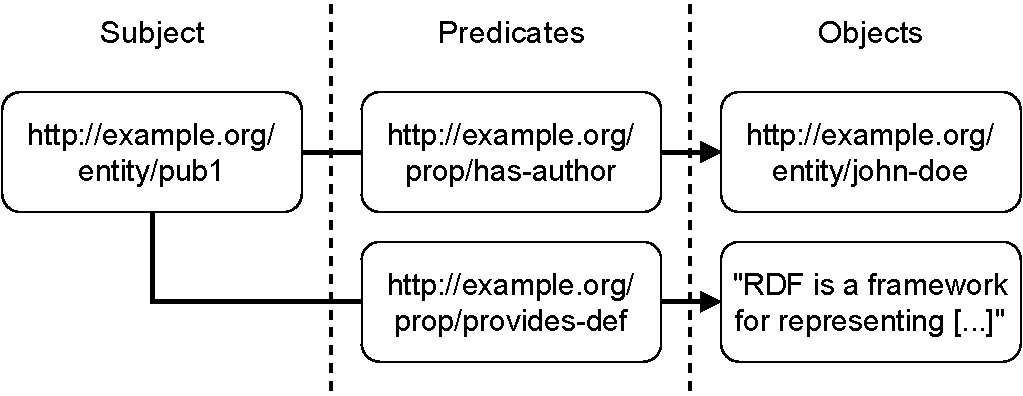
\includegraphics[max width=0.7\columnwidth]{./figures/triple_example}
\caption{A simple exemplary knowledge graph consisting of two RDF triples. The upper triple provides contextual information, the lower triple contentual information of the publication \emph{{pub1}}. All non-literal triple members are identified using IRIs. (Figure and caption adopted from~\cite{Martin21}.)}
\label{fig:contentual-contextual}
\end{figure}

\Cref{fig:contentual-contextual} shows an imported figure.

\subsection*{Experimental Result Import}

\subsection*{Software Import}

